%Chapter 7

\chapter{Tools} % Main chapter title

\label{tools} % For referencing the chapter elsewhere, use \ref{Chapter1} 

\lhead{Chapter 7. \emph{Tools}} % This is for the header on each page - perhaps a shortened title

%----------------------------------------------------------------------------------------
This chapter discussed the tools and data sets used, it starts by section ~\ref{pre} which discusses the pre-processing tools used, sections ~\ref{lucene}, ~\ref{awn} and ~\ref{crawlers} demonestrates the usage of \textit{lucene}, \textbf{A}rabic \textbf{W}ord \textbf{N}et (AWN), section ~\ref{corpus} discusses the data sets used, finally section ~\ref{lsa} shows the tools used to implement \textit{LSA}.
\section{Text Preprocessing}\label{pre}
There has been a debate among researchers about the benefits of using morphological tools in Text Analysis. Studies in the \textit{English}
language illustrated that performing stemming during the preprocessing step degrades the performance slightly \citep{pre_8} \citep{pre_9}. 
In this work, the preprocssing consists of three steps: First stop words are removed, second a part of speech tag is assigned to each term and then each term is stemmed.
The output of the preprocessing module is the stem of each term concatenated with its part of speech, to distinguish between noun and verb. for example this sentence "\RL{مجلس الأمن يدرس بياناً يدعو إلى رفع الحصار واقتراح أوروبي}" is mapped to (\RL{مجلس}n, \RL{أمن}n, \RL{يدرس}v, \RL{بيانا}n, \RL{يدعو}v, \RL{رفع}n, \RL{حصار}n, \RL{اقتراح}n, \RL{أوروب}n).

In this work two different techniques are used for stemming: Elkhoja stemmer and Light stemming.

\subsection{Part of speech tagging}

The part of speech tagging is defined as  the process of marking up a word in a text (corpus) as corresponding to a particular part of speech, based on both its definition, as well as its contexti.e. relationship with adjacent and related words in a phrase, sentence, or paragraph. 
Stanford Log-linear Part-Of-Speech Tagger \citep{pre_1} \citep{pre_2} is used to tag each term in the document.


\subsection{Stemming}
Stemming is the process of removing all of a word's prefixes and suffixes to produce the stems or the root \citep{pre_3}.
The experiment conducted by \citep{pre_10} indicates that using stemming and dimensionality reduction techniques is not necessary. On the other hand Arabic language is highly derivative where tens or even hundreds of words could be
formed using only one root. The importance of the stemming process comes in the classification and index builders/searchers because it makes the operations fewer dependants on particular form of words, and it reduces the potential size of vocabularies which might otherwise have to contain all possible forms.
Furthermore, a single word may be derived from multiple roots (Attia, 2000). 

Arabic stemming algorithms can be classified, according to the desired level of analysis, as either: 
(a)stem-based or (b)root-based algorithms. Stem-based algorithms, remove prefixes and suffixes from Arabic words, while root-based algorithms reduce stems to roots. After stemming the stem may be further processed to compass the word root in the root-based approach (Darwish, 2003). 
As an example, the stem of “Ketabhom (their book)” is “Ktab (book)” and its root is “Ktb (wrote)” while the stem of the word “Ktateeb
(places for learning Quran)” is the same word “Ktateeb” but the root is  “Ktb (wrote)”.

Early studies performed on IR indicated that using root words is better than using stemmed words as mentioned by (Darwish, 2003). Other studies, by \citep{pre_11} (Moukdad, 2006), reported that the stem-based approach is superior to the root-based approach. An experiment performed by (Darwish et al., 2005) showed that using context to improve the root extraction process may enhance the process of IR slightly compared to the stem-based approach. However, the context root extraction is computationally expensive compared with the stemming. On the contrary, Brants et al. (Brants et al., 2002) reported that performing stemming to the Arabic text increases the ambiguity, and hence using the raw text may be better.



The performance of information retrieval in arabic language is very problematic due to the specific morphological and structural changes in the language: polysemy, irregular and inflected derived forms, various spelling of certain words, various writing of certain combination character, short (diacritics) and long vowels, most of the arabic words contain affixes figures ~\ref{fig:pre_3} ~\ref{fig:pre_4}. To address these problems, several methods have been proposed.
The vocabulary of the arabic language is essentially built from the roots derivation. The roots are words composed of three to five consonants letters. The arabic language has about ten thousand roots, 85\% of them are trilateral. The derivation of words is done by adding affixes (prefix, infix, or suffix) to the root according to several patterns that are around 120 (Al Kharashi, 1999). For example, let us take the root (\RL{كتب}); the words (\RL{كاتب}, \RL{كاتبه},\RL{مكتوب}).
Before applying stemming , the normalization phase is applied before applying these methods, the text normalization takes a character string as input and tries to remove or replace some characters under the predefined rules to converts it into a string of letters (Figure ~\ref{fig:pre_1}).

\begin{figure}[htbp]
	\centering
		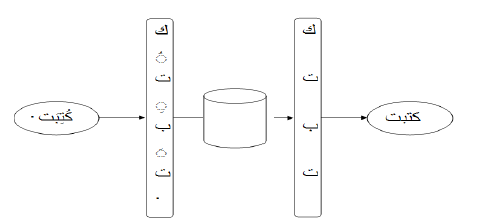
\includegraphics{./Figures/pre_1.png}
		\rule{35em}{0.5pt}
	\caption[Normalization for Arabic text.]{Normalization for Arabic text.}
	\label{fig:pre_1}
\end{figure}

\begin{figure}[htbp]
	\centering
		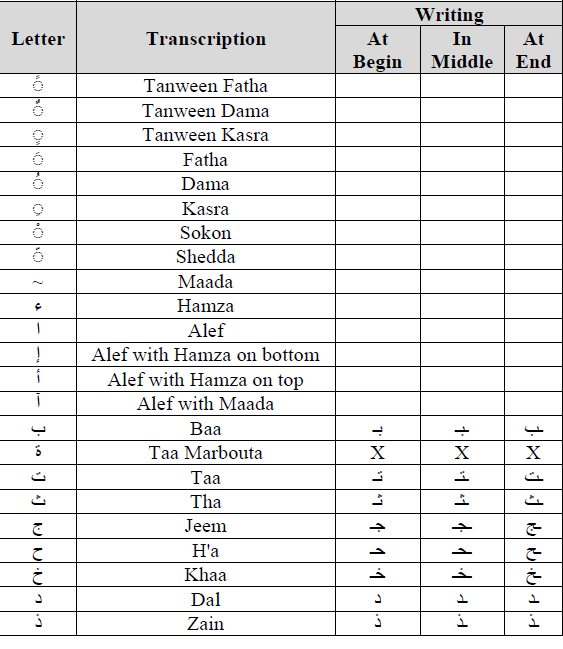
\includegraphics{./Figures/pre_3.png}
		\rule{35em}{0.5pt}
	\caption[Arabic affixes.]{Arabic affixes.}
	\label{fig:pre_3}
\end{figure}

\begin{figure}[htbp]
	\centering
		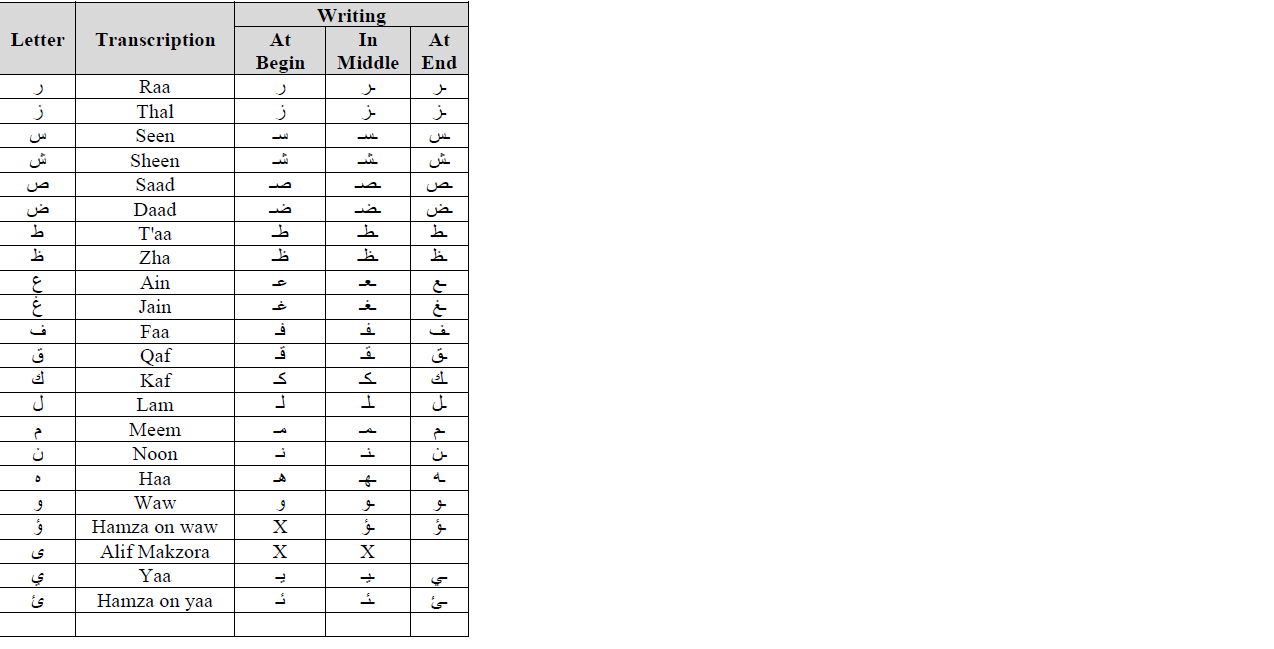
\includegraphics{./Figures/pre_4.png}
		\rule{35em}{0.5pt}
	\caption[Arabic affixes.]{Arabic affixes.}
	\label{fig:pre_4}
\end{figure}

The two components (POS and stemmer) are combined in to one larger component where the document is passed to it and two arrays are returned one contains the part of speech tag while the other stores the stem. The stemming must be perofmed after the POS, because stemming may affect the POS results.

\subsubsection{Stemming based on pattern and affixes}
Arabic patterns are part of the Arabic grammar. They are formed based on the Arabic root \citep{pre_4}. A
root is the base form of a word which can not be further analyzed without the loss of the word's
identity, or it is that part of the word left when all the affixes are removed.
An Arabic root is an ordered sequence of three (\RL{فعل}) or four letters (\RL{فعلل}) from alphabet \citep{pre_5}. The
root has a general, basic meaning which forms the basis of many related meanings. These related
meanings are represented by the root consonants put in different forms called patterns \citep{pre_6}. They
are generated from the process of vocalization and affixation \citep{pre_20}. Table 1 shows a sample of the
Arabic Patterns (Three-Consonant root).
Variations of the root and patterns determine the actual meaning of the word. For example, the
root (\RL{كتب}) with the addition of the letter (\RL{ا}) gives the word (\RL{كتاب}), which means book, while the root pattern combination of 
(\RL{كاتب}) means "one who writes" or "clerk". There are
also some prefixes and suffixes which determine whether a word is a subject marker, pronoun,
preposition, or a definite article. Figure ~\ref{fig:pre_5} and ~\ref{fig:pre_6} illustrates set of derivatives patterns, its corresponding
English word, the position in the language and its Arabic patterns from the Arabic trilateral verbal
root \RL{كتب} (k t b).


\begin{figure}[htbp]
	\begin{center}
		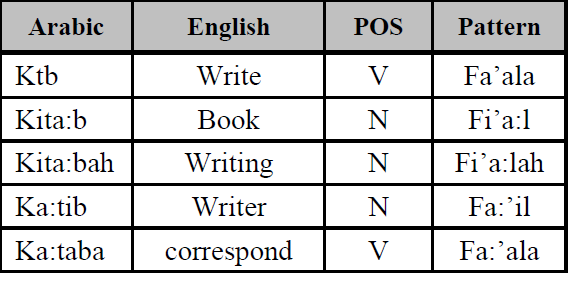
\includegraphics{./Figures/pre_5.png}
		\rule{20em}{0.001pt}
	\end{center}
	\caption[Derivatives of the Arabic trilateral root ‘k t b’.]{Derivatives of the Arabic trilateral root ‘k t b’.}
	\label{fig:pre_5}
\end{figure}

\begin{figure}[htbp]
	\begin{center}
		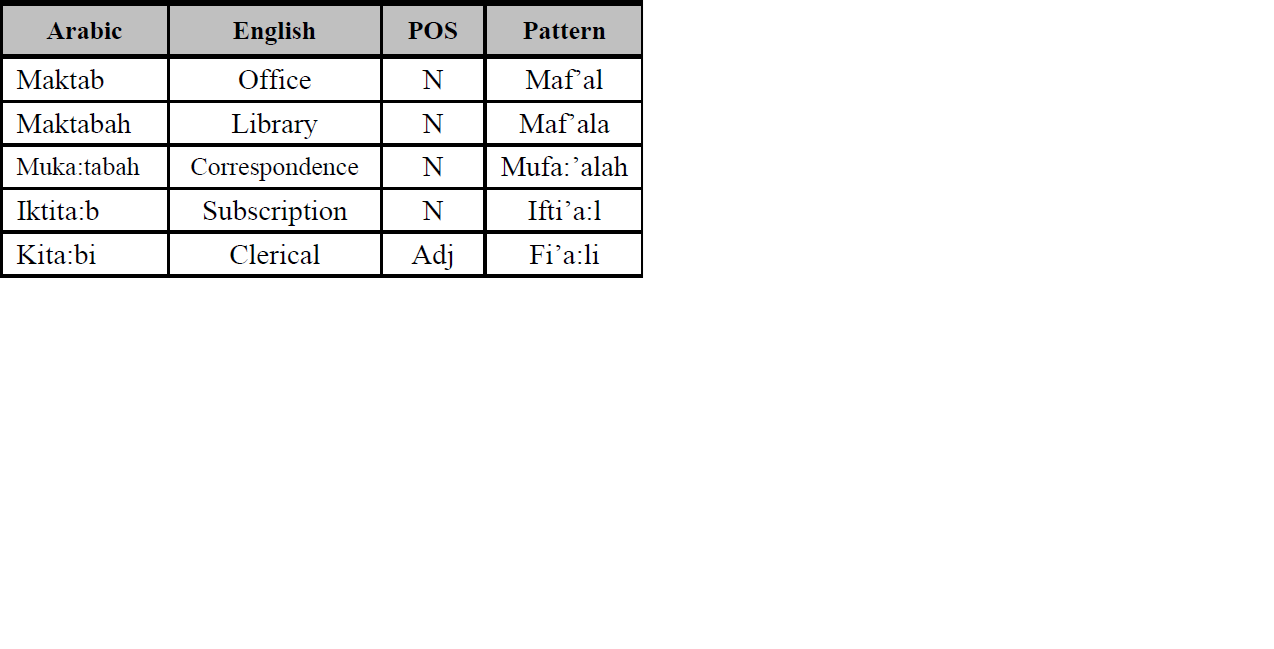
\includegraphics{./Figures/pre_6.png}
		\rule{20em}{0.001pt}
	\end{center}
	\caption[Derivatives of the Arabic trilateral root ‘k t b’.]{Derivatives of the Arabic trilateral root ‘k t b’.}
	\label{fig:pre_6}
\end{figure}


Stemmer based on pattern and affixes Several Stemmer algorithms based on the patterns and affixes have been developed, to find roots with three letters, four and five letters, starting from verbal forms, nouns and adjectives derived from verbs S. Khoja and R. Garside (1999) have proposed a method that involves removing diacritics representing vowelization, the stop words, the punctuation, the numbers, the definite article (\RL{ال}), the inseparable conjunction (\RL{و}), and the longest prefix and suffix. Then, the result is compared to a list of patterns. If a match is found, the characters representing the root in the pattern are extracted.
\subsubsection{Arabic Light Stemmers}
It is not an aggressive practice as the root-based algorithm. The aim of this approach is not to produce the linguistic root of a given Arabic surface form; rather, it is to remove the most frequent suffixes and prefixes.
In Arabic, unlike English, both prefixes and
suffixes are removed for efficient results, but Arabic provides the additional difficulty of infixes
[24]. The difficulty arises because Arabic has two genders, feminine and masculine; three
cardinality, singular, dual, and plural; and three grammatical cases, nominative, genitive, and
accusative. A noun has the nominative case when it is a subject; accusative when it is the object
of a verb; and genitive when it is the object of a preposition. The form of an Arabic noun is
determined by its gender, cardinality, and grammatical case. Light Stemmers remove only prefixes and suffixes. Five pre-defined groups of removable
prefixes and suffixes were offered.

\section{Lucene}\label{lucene}
\label{luceneTool}
Apache Lucene(TM) is a high-performance, full-featured text search engine library written entirely in Java. It is a technology suitable for nearly any application that requires full-text search, especially cross-platform.
\begin{figure}[htbp]
	\begin{center}
		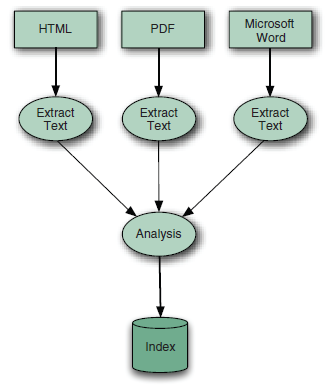
\includegraphics{./Figures/lucene.png}
		\rule{20em}{0.5pt}
	\end{center}
	\caption[Lucene Indexing Process]{Lucene Indexing Process}
	\label{fig:lucene1}
\end{figure}
\begin{figure}[htbp]
	\begin{center}
		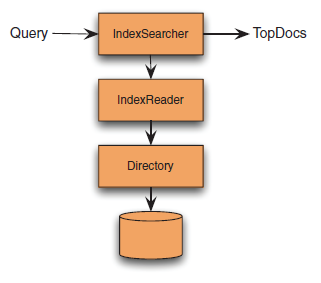
\includegraphics{./Figures/lucene_search.png}
		\rule{20em}{0.5pt}
	\end{center}
	\caption[Lucene searching Process]{Lucene searching Process}
	\label{fig:lucene2}
\end{figure}
Apache Lucene is an open source project available for free download. Please use the links on the right to access Lucene.
Features
Lucene offers powerful features through a simple API:\\
Scalable, High-Performance Indexing
\begin{itemize}
   \item over 95GB/hour on modern hardware
   \item small RAM requirements -- only 1MB heap
  \item  incremental indexing as fast as batch indexing
    \item index size roughly 20-30% the size of text indexed
\end{itemize}
Powerful, Accurate and Efficient Search Algorithms
\begin{itemize}
 \item   ranked searching -- best results returned first
  \item  many powerful query types: phrase queries, wildcard queries, proximity queries, range queries and more
  \item  fielded searching (e.g., title, author, contents)
 \item   date-range searching
   \item sorting by any field
  \item  multiple-index searching with merged results
  \item  allows simultaneous update and searching
\end{itemize}
Cross-Platform Solution
\begin{itemize}
  \item  Available as Open Source software under the Apache License which lets you use Lucene in both commercial and Open Source programs
 \item   100%-pure Java
  \item  Implementations in other programming languages available that are index-compatible
\end{itemize}
\textit{The Apache Software Foundation}\\

The Apache Software Foundation provides support for the Apache community of open-source software projects. The Apache projects are defined by collaborative consensus based processes, an open, pragmatic software license and a desire to create high quality software that leads the way in its field. Apache Lucene, Apache Solr, Apache PyLucene, Apache Open Relevance Project and their respective logos are trademarks of The Apache Software Foundation. All other marks mentioned may be trademarks or registered trademarks of their respective owners.\\
\section{AWN}\label{awn}
Arabic WordNet is the Arabic analogue to the widely used WordNet for the English language. The Arabic WordNet (AWN) is a lexical database of the Arabic language following the development process of Princeton English WordNet and Euro WordNet. It utilizes the Suggested Upper Merged Ontology as an interlingua to link Arabic WordNet to previously developed wordnets. Christiane Fellbaum at Princeton was the project lead. The project was sponsored by DOI/REFLEX.\\
From http://www.globalwordnet.org/AWN/DataSpec.html you can get the XML data exchange specifications of the database. AWN contains about 11,000 synsets (including 1,000 NE).\\

There are several different ways for accessing the database:\\
\begin{itemize}
\item[1] The browser package (available at http://sourceforge.net/projects/awnbrowser/) includes the AWN data and Princeton WN2.0 mappings in a relational database. You can use the export facilities to export the data as XML or CSV to taylor them to your needs .\\
\item[2] The database can also be downloaded in XML format (linked to Princeton WN 2.0) from \url {http://nlp.lsi.upc.edu/awn/get_bd.php}\\
\item[3] A set of basic python functions for accessing the database can be obtained from: \url {http://nlp.lsi.upc.edu/awn/AWNDatabaseManagement.py.gz}\\
\end{itemize}
Functionality:\\
\begin{itemize}
\item AWN Browser: Browsing the database\\
\item AWN can be downloaded in XML format and access its content be directly used at developers' will.\\
\end{itemize}
Technology:\\
    Java, Perl, MySQL\\
Innovation:\\
	One of the most important lexical resources for Arabic language.\\
\begin{figure}[htbp]
	\begin{center}
		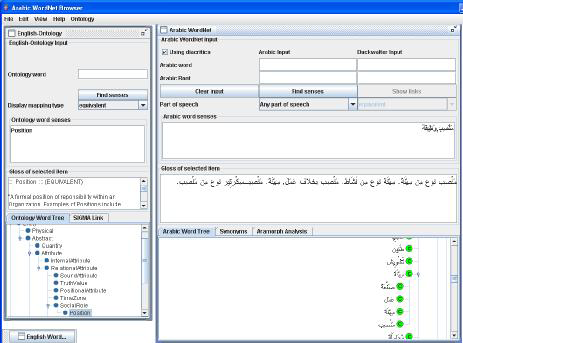
\includegraphics{./Figures/AWNGUI.png}
		\rule{20em}{0.5pt}
	\end{center}
	\caption[AWN GUI]{AWN GUI}
	\label{fig:AWN GUI}
\end{figure}
\begin{figure}[htbp]
	\begin{center}
		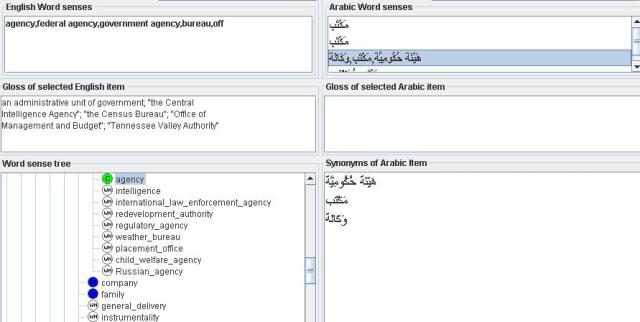
\includegraphics{./Figures/AWNGUI_1.jpg}
		\rule{20em}{0.5pt}
	\end{center}
	\caption[AWN GUI]{AWN GUI}
	\label{fig:AWN GUI}
\end{figure}
%-----------------------------------------------------------------------------------------

\section{Crawlers}\label{crawlers}
we used Web-Harvest for web pages crawling and retrieving the desired data.It’s an Open Source Web Data Extraction tool written in Java. It offers a way to collect desired Web pages and extract useful data from them. In order to do that, it leverages well established techniques and technologies for text/xml manipulation such as XSLT, XQuery and Regular Expressions. Web-Harvest mainly focuses on HTML/XML based web sites which still make vast majority of the Web content. On the other hand, it could be easily supplemented by custom Java libraries in order to augment its extraction capabilities.
Process of extracting data from Web pages is also referred as Web Scraping or Web Data Mining. World Wide Web, as the largest database, often contains various data that we would like to consume for our needs. The problem is that this data is in most cases mixed together with formatting code - that way making human-friendly, but not machine-friendly content. Doing manual copy-paste is error prone, tedious and sometimes even impossible. Web software designers usually discuss how to make clean separation between content and style, using various frameworks and design patterns in order to achieve that. Anyway, some kind of merge occurs usually at the server side, so that the bunch of HTML is delivered to the web client.
Web-Harvest is distributed under BSD License. It gives the freedom for anyone to use, explore, modify, and distribute Web-Harvest, but without any warranty. 
\subsection{Basic concept}
The main goal behind Web-Harvest is to empower the usage of already existing extraction technologies. Its purpose is not to propose a new method, but to provide a way to easily use and combine the existing ones. Web-Harvest offers the set of processors for data handling and control flow. Each processor can be regarded as a function - it has zero or more input parameters and gives a result after execution. Processors could be combined in a pipeline, making the chain of execution. For easier manipulation and data reuse Web-Harvest provides variable context where named variables are stored. The following diagram describes one pipeline execution:

\begin{figure}[htbp]
	\centering
		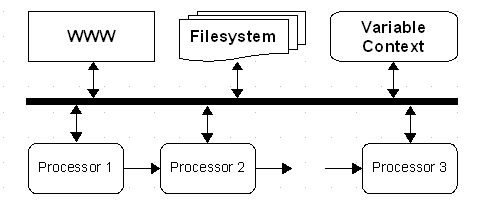
\includegraphics{./Figures/diagram1.png}
		\rule{35em}{0.5pt}
	\caption[Web-Harvest]{Web-Harvest}
\end{figure}


The result of extraction could be available in files created during execution or from the variable context if Web-Harvest is programmatically used.
Configuration language

Every extraction process is defined in one or more configuration files, using simple XML-based language. Each processor is described by specific XML element or structure of XML elements. For the illustration, here is presented an example of configuration file:
you may check the XML configuration file here \ref{crawlersXML}

This configuration contains two pipelines. The first pipeline performs the following steps:
\begin{itemize}
\item [1] HTML content at http://news.bbc.co.uk is downloaded
\item [2] HTML cleaning is performed on downloaded content producing XHTML,
\item [3] XPath expression is searched for, giving URL sequence of page images,
\item [4] New variable named "urlList" is defined containing sequence of image URLs.
\end{itemize}
The second pipeline uses result of the previous execution in order to collect all page images:
\begin{itemize}
\item [1] Loop processor iterates over URL sequence and for every item:
\item [2] Downloads image at current URL,
\item [3] Stores the image on the file system.
\end{itemize}


\section{Corpus}\label{corpus}
We used two corpora one of them is Al Jazeera, which contains 4462 article from various categories like Arts,culture,Economy, International, locals, Medical, Society, Sport.
The other corpus is upto-date corpus extracted using crawling tool with predefined XML files from specific News agency Like: Reuters, CNN, BBC, Al Arabiya, Youm7.This corpus was around 160 articles from many categories.


\section{LSA Tools}\label{lsa}
\subsection{Python}
\subsubsection{Description}
Python is a remarkably powerful dynamic programming language that is used in a wide variety of application domains. Python is often compared to Tcl, Perl, Ruby, Scheme or Java. Some of its key distinguishing features include:
\begin{itemize}
\item very clear, readable syntax
\item strong introspection capabilities
\item intuitive object orientation
\item natural expression of procedural code
\item full modularity, supporting hierarchical packages
\item exception-based error handling
\item very high level dynamic data types
\item extensive standard libraries and third party modules for virtually every task
\item extensions and modules easily written in C, C++ (or Java for Jython, or .NET languages for IronPython)
\item embeddable within applications as a scripting interface
\end{itemize}
\subsubsection{Usage}
Python was used as the main programming language for the LSA implementation due to being extensible till the Ram size and having many third party packages for haonendling SVD calculations
\subsection{DIVISI2}
\subsubsection{Description}
Divisi is a sparse SVD toolkit for Python that is particularly designed for working with semantic networks.
\subsubsection{Usage}
Divisi was used to calculate SVD in a sparse way as the term vs. document matrix is so sparse so sparse SVD is more efficient than normal one
\subsection{PyTables}
\subsubsection{Description}
PyTables is a package for managing hierarchical datasets and designed to efficiently and easily cope with extremely large amounts of data. 
PyTables is built on top of the HDF5 library, using the Python language and the NumPy package. It features an object-oriented interface that, combined with C extensions for the performance-critical parts of the code (generated using Cython), makes it a fast, yet extremely easy to use tool for interactively browse, process and search very large amounts of data. One important feature of PyTables is that it optimizes memory and disk resources so that data takes much less space (specially if on-flight compression is used) than other solutions such as relational or object oriented databases.
\subsubsection{Usage}
PyTables was used to save the term vs. document matrix in a h5 file format which caches part of the array in the Ram so as to be able to deal with array sizes bigger than that of the Ram. Also, the array is saved in a compressed format.
\subsection{Numpy}
\subsubsection{Description}
NumPy is the fundamental package for scientific computing with Python. It contains among other things:
\begin{itemize}
\item a powerful N-dimensional array object
\item sophisticated (broadcasting) functions
\item tools for integrating C/C++ and Fortran code
\item useful linear algebra, Fourier transform, and random number capabilities
\end{itemize}
Besides its obvious scientific uses, NumPy can also be used as an efficient multi-dimensional container of generic data. Arbitrary data-types can be defined. This allows NumPy to seamlessly and speedily integrate with a wide variety of databases.
\subsubsection{Usage}
Numpy was used to perform matrix operations like: calculating the cosine similarity, calculate the vector representation of the document.


